\chapter{\sffamily Centralised exchanges}

{\bfseries\sffamily Concept.} To define and develop an archetype simulation environment for centralised exchanges. In our classification scheme, this archetype is defined by a bidirectional star state partition graph topology and would make sense for simulations of financial, betting and housing markets as well as other forms of resource exchange. We will also discuss the typical ways in which the state partitions of the system may only partially be observed in realistic examples, and analyse how best to deal with each situation. For the mathematically-inclined, this chapter will define the mapping of our formalism to centralised exchanges. For the programmers, the software which is designed and described in this chapter can be found in the public Git respository here: \href{https://github.com/worldsoop/worldsoop}{https://github.com/worldsoop/worldsoop}.

\section{\sffamily Defining the archetype}

The centralised exchange archetype refers to simulation environments with a very specific bidirectional state partition graph topology. The graph connection structure is a star configuration where every state partition is connected to the same, centralised state partition which itself has a unique function in the model. In case this description isn't that clear, we've added an illustration of the graph for this archetype in Fig.~\ref{fig:state-partition-graph-centralised-exchanges}.

\begin{figure}[h]
\centering
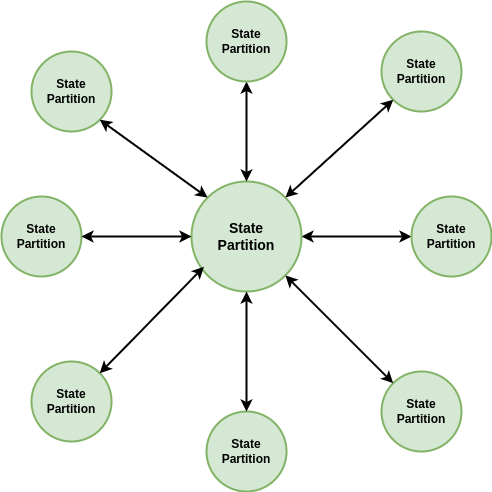
\includegraphics[width=9cm]{images/chapter-10-state-partition-graph.drawio.png}
\caption{State partition graph topology for centralised exchange archetypes.}
\label{fig:state-partition-graph-centralised-exchanges}
\end{figure}

Before moving on to discuss how data is typically collected for centralised exchanges, it will be informative to list the examples of phenomena where this archetype can be found in the real-world. These problem domains are:
%%
\begin{itemize}
\item{Financial~\cite{fischer2018reinforcement,meng2019reinforcement} and sports betting~\cite{cliff2021bbe} market simulations for developing algo-trading strategies and portfolio optimisation~\cite{dangi2013financial}, as well as housing market simulations~\cite{yilmaz2018stochastic,carro2023heterogeneous} to evaluate government policies.}
\item{Simulations of other forms of resource exchange through centralised mediation, such as in prosumer energy markets~\cite{may2023multi}.} 
\end{itemize}
%%

\textcolor{red}{Within this topological archetype there will also be other categories to think are applicable:
\begin{itemize}
\item{Types of observation that can be made about the state.}
\item{Types of action that can be taken by an agent.}
\item{Types of agent? How frequently do these actions get taken? On what part of the state?}
\end{itemize}
}

\section{\sffamily Writing the code}
